\documentclass[../thesis.tex]{subfiles}

\chapter{Background}\label{background}
This chapter presents the background and theory relevant to this thesis.
First I will give a brief introduction to the field of vocal programming
and some of the challenges associated with it.
Second, the tools and techniques that will be used
to address these challenges will be presented.
Lastly, there will be an introduction to the Elm
programming language, which will be the subject
of the experiments presented in \Vref{the_project}.
% In this section I will cover the history of voice coding (Dragon, NatLink, Dragonfly, Caster etc\ldots)
% as well as the state of the art language tooling. (LSP and TreeSitter).
% I will also cover something about the Elm programming language, as I will be using that in my analysis.

% \section{Accessibility}%
% \label{sec:accessibility}

\section{Vocal Programming}

Vocal programming is a complex field with many interesting challenges.
Users need to be able to dictate and edit code, navigate files, as well as being able to perform a plethora
of other tasks such as compiling and running the code, and use version control.
This section provides a brief introduction, while Chapter~\ref{talon}
provides a more in-depth explanation to how people are using Talon to program.

\subsection{History}

\paragraph{Dragon NaturallySpeaking}
was the worlds first large-vocabulary general purpose dictation system.
Dragon is in many ways the foundation for many of tools like Talon.
Some voice systems use it as just a speech engine, but it also provides other functionality like mouse control.
It is available for Mac and Windows, but the product has been discontinued for Mac.% when??
Mac users who would like to use Dragon can still purchase it online, and it still works.
% The mac version is still available on eBay, and still works. % maybe something here about the download stuff.

\paragraph{NatLink:}
While Dragon alone is a very powerful dictation system, it's customization ability is limited.
Dragon does provide a simple scripting language in the pro edition, but it has very limited capabilities compared to
modern general purpose scripting languages.
In 1999, NatLink was developed to address this problem. 
It is a macro system for Dragon which lets the user write scripts that can be triggered by voice commands
in Python~\parencite{gould2001implementation}.
Later on, more high-level APIs were built on top on NatLink such as Dragonfly. % Not really precise. Need to look into history here.

\paragraph{}
These technologies heavily influenced modern voice control systems such as Talon,
many of which still support Dragon as the speech recognition engine.
In 2013, Travis Rudd held a talk at PyCon demonstrating the power
of vocal programming\footnote{Using Python to Code by Voice: \url{https://www.youtube.com/watch?v=8SkdfdXWYaI}}.
This talk was very influential and was for many people
their first exposure to the field.




% \paragraph{Dragonfly}
% Higher-level scripting api on top of natlink.

% \paragraph{Caster}
% Another layer on top of dragonfly. Not totally sure if worth discussing.

% \paragraph{VoiceCode}
% Seems like this was a popular dictation system at some point. There are papers on it, so might be worth discussing.

\subsection{Dictation}
Dictation, in this context, is the act of speaking phrases into a microphone and have those phrases translated into text.
This is made possible by a technique called \textit{Speech Recognition} which combines techniques from natural language processing
and signal processing. The sound waves from the user is captured by the microphone, processed, and sent off to a machine learning algorithm
that will try to fit the input into a sequence of words, or a sentence, in the target language (i.e English). Speech recognition
has been around for a while, but has just in the past decade seeing huge boosts in accuracy, partly due to the advancements in deep learning.
Voice controlled applications are built on top of programs implementing the speech recognition, often referred to as \textit{Speech Recognition Engines}.

Beyond the technical aspect, efficient dictation also requires a great deal of attention from the user.
To achieve high accuracy while dictating, it is not sufficient, or at least not optimal, to simply speak as one normally would.
New users will have to practice things like speaking at a consistent pace and volume, and being aware of their distance to the microphone (to try not to vary too much).
Some users will also need to enunciate their words much more than they are used to, especially if they are not native speakers of the language in which they are dictating.
Different users can experience very different results with the same engine simply due to a high degree of variation between peoples voices.
Users also need to configure and personalize the system by adding words to the vocabulary of the engine, and training the engine on words that they are
having a hard time getting recognized. This process is often very incremental, and optimal results might not be achieved until the user has
use the system for a while.

People not used to dictating will also experience a high degree of cognitive load in the beginning, which will slow down their work.
Dictation is usually more accurate when the user speaks in full sentences, as opposed to single words, or even short phrases.
Users will therefore have to learn to plan out their sentences before starting to speak.
This can feel very different from the experience of typing on a keyboard, but it is a challenge that is surmountable by practice.

% \paragraph{Command First vs Data First}
% Two different dication strategies.
% Command first = Output only triggered when a command is triggered by speaking a particular phrase.
% Data first = The user can speak without keywords. The system should infer capitalization and punctuation.
% Here i will describe the tradeoff between these two.

\paragraph{Homophones}
are words that sound the same as another word, but have different meaning.
These groups of words may be spelled the same or differently.
For example, ``rose'' may refer to the past tense of rise, or the flower.
The word ``pair'' is \textit{homophonic} to ``pear'', and ``pare''.
Homophones that are also spelled the same are also known as homographs, whereas the ones spelled differently are called heterographs.
In the context of vocal programming, and speech recognition in general, we are only interested in heterographs as we do not consider
the underlying meaning of a phrase beyond whether or not it was what the user intended to input.
Although we are only considering this subset, I will be using the more general term homophone as this is more widely used in the 
Talon community.
% documentation
% of the system I will be discussing.

Homophones are a very big challenge for vocal programming,
as speech recognition engines are not able to reliably distinguish between them.
Often they can still infer the correct word based on the context in which it was used.
For example, Dragon can reliably recognize the phrase ``I saw that with my eye'' correctly despite the fact that ``I'' and ``eye'' are homophonic.
However, if they are not spoken within a sentence, they cannot be distinguished on the user will likely see only one of the options every time.
This problem is a bigger challenge for vocal programing than prose dictation because program text is not formed by English sentences, and more words needs to be
spoken one at a time.

There are however techniques for alleviating this problem, which will be discussed in \Vref{dealing_with_homophones}.


\section{Structural Editing}
Structural editing is a technique used by some code editors to allow users to directly manipulate the underlying structure of the program.
Computer programs typically have a textual representation that is readable both by humans and compilers.
When a compiler reads a program, the text is converted to a data type known as the \textit{Abstract Syntax Tree} (AST), during the parsing phase.
The AST contains all the information about the program necessary to produce the executable output program.
When modifying a program the desired outcome is always a correct change in the underlying AST, however it is not always
trivial to map of single text transformation to a transformation on the AST.
One of the goals of structural editing is to allow users to work on a higher abstraction level.
Another is to reduce the amount of invalid states the program needs to go through
before the desired modification is completed.
For this reason it is a popular technique in editors designed specifically for beginners.
One very well-known example is \textit{Scratch} which is an educational tool for teaching children to code.
It provides a drag-and-drop interface enriched with visual cues that makes it easy to
put together structurally valid programs.
Scratch is an example of a purely structure oriented code editor.
It does not provide a text based interface to the language.
There are also hybrid approaches that adds a structural layer on top of a normal text based editor.
These editors are sometimes referred to as structure-aware editors.

\paragraph{}

Despite having some clear advantages over traditional text based editors, structural editors are not commonly used among professional developers.
One reason for this is that the editors that are popular today have many years of engineering behind them.
There are no structural editors that come close in the amount of features or polish to that of IntelliJ, VSCode or Vim.
Structural editor still have unresolved issues in their design that needs to be addressed before they will see commercial use.
One example of a more advanced structural editor is
``Deuce'', which is a structure-aware editor developed as part of a research project at the University of Chicago~\parencite{deuce}.
It suggests a hybrid approach that addresses some of the problems with current text based work-flows.
% I will be using this as a reference for what the modern structural editor might look like.

% \section{PL Theory}
% As much of the work is related to analysing programs, I should cover some general stuff abuut languages.
% Not sure how much detail is appropriate here, but could be a source for a lot of content.
% Possible subjects: Parsing, type checking/inference, scopes, etc.

\section{Language Server Protocol}
Programmers today expect more of their code editing software than the ability to edit text.
Integrated Development Environments (IDE) such as \textit{Intellij} and \textit{Eclipse} support many language specific features such as \textit{go to definition}, \textit{re-factoring}
and displaying where the errors are in the program.
Implementing these features take significant effort as they require the implementation of a large portion of the language front-end.
This makes it very difficult for a new language to gain support across different IDEs.
The solution is to decouple the language support from the editors by moving to code that does program analysis to an external program (server).
The Language Server Protocol defines how these servers communicate with code editors.

\subsection{Client/Server Communication}%
\label{sub:client_server_communication}
Clients (editors) and servers communicate over JSON-RPC, which is a remote procedure call protocol encoded in JSON.
This allows clients to notify servers without having to wait for a response, on the server can respond to multiple requests asynchronously.
The format of the messages sent between server and client can be seen in \Vref{listing:jsonrpc}, and
an illustration of how clients and servers communicate during a normal editing session can be seen in \Vref{fig:lsp-communication}
\footnote{\url{https://microsoft.github.io/language-server-protocol/overviews/lsp/overview/}}.
% Messages between the server and client will have the following form:

\begin{listing}[ht]
\begin{Verbatim}
Content-Length: ...\r\n
\r\n
{
	"jsonrpc": "2.0",
	"id": 1,
	"method": "textDocument/didOpen",
	"params": {
		...
	}
}
\end{Verbatim}
\caption{JSON-RPC Example}
\label{listing:jsonrpc}
\end{listing}


\begin{figure}[htpb]
    \centering
    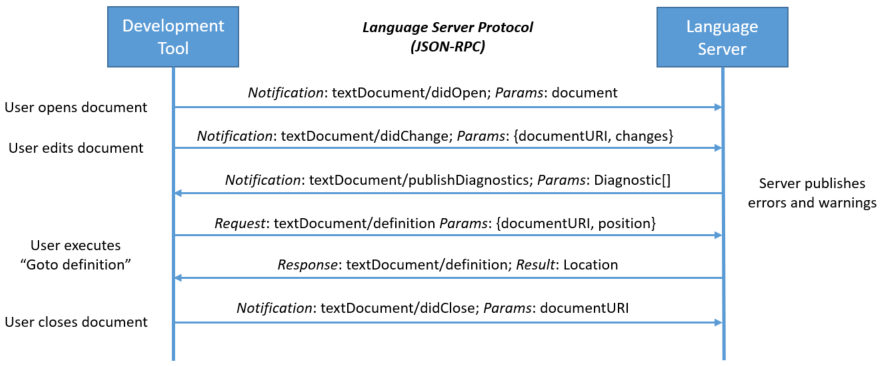
\includegraphics[width=1\linewidth]{images/lsp-communication.png}
    \caption{Example Communication During Editing Session}%
    \label{fig:lsp-communication}
\end{figure}

\section{TreeSitter}
TreeSitter is a parser generator tool and an incremental parsing library~\parencite{WinNT}.
It was conceived as a solution to the problem of quick semantic syntax highlighting,
but is also used in the implementation of some language servers.
An incremental parser is one that can update the parse tree without having to re-parse the entire
file with each modification~\parencite{incremental}.
Parser produced by TreeSitter are failure tolerant, which means that the parser will not instantly reject
programs with syntax errors.
This is a crucial feature for editors because the programs being analyzed
are in an incomplete state a large portion of the time.

There are currently parsers written for many different languages.
Because TreeSitter provides such excellent syntax highlighting, developers are incentivized
to create and maintain parser for their language, even if the language
uses a different parser for the compiler.
TreeSitter can therefore be used as a common parsing framework for any tool that need to
handle many different programming languages.

\subsection{Libraries and Bindings}%
\label{sub:libraries_and_bindings}
TreeSitter produces parsers in pure \textit{C}.
Documentation for the C API can be found on the official website.
There are also bindings to the C API for a few different languages.
The official TreeSitter repository include bindings for Rust, as well as
JavaScript (Web Assembly and NodeJS), Python, Ruby and Haskell.
The bindings for Rust are the most mature and well-documented.
Out of the other bindings, the ones for JavaScript and Python are the most complete.
% mention that Ruby and Haskell does not have a query support?

\subsection{Using Parsers}%
\label{sub:using_parsers}
To use TreeSitter, simply install the library along the individual parsers for each language you would like to parse.
This process varies depending on which bindings are being used.
For the NodeJS bindings, both the library and parser can be installed via NPM:
\begin{minted}{bash}
npm install tree-sitter
npm install tree-sitter-javascript
\end{minted}
Listing~\ref{listing:tsexample} shows a JavaScript program that uses TreeSitter to parse a JavaScript program and simply print the parse tree
as an S-expression.
The result of running the above program can be seen in Listing~\ref{listing:tsexresult}.

\begin{code}{JavaScript}{Simple TreeSitter Example}{listing:tsexample}
    
const Parser = require('tree-sitter');
const JavaScript = require('tree-sitter-javascript');

const parser = new Parser();
parser.setLanguage(JavaScript);

const sourceCode = 'x = 5';
const tree = parser.parse(sourceCode);

console.log(tree.rootNode.toString());
\end{code}
\begin{code}{text}{Result from running Listing~\ref{listing:tsexample}}{listing:tsexresult}
(program 
  (expression_statement 
    (assignment_expression 
      left: (identifier) 
      right: (number))))
\end{code}

The website also provides an interface for interacting with the library
that visualizes the parse tree as the program changes\footnote{\url{https://tree-sitter.github.io/tree-sitter/playground}}.
The same example can be seen in Figure~\ref{fig:playground}. 

\begin{figure}[htpb]
    \centering
    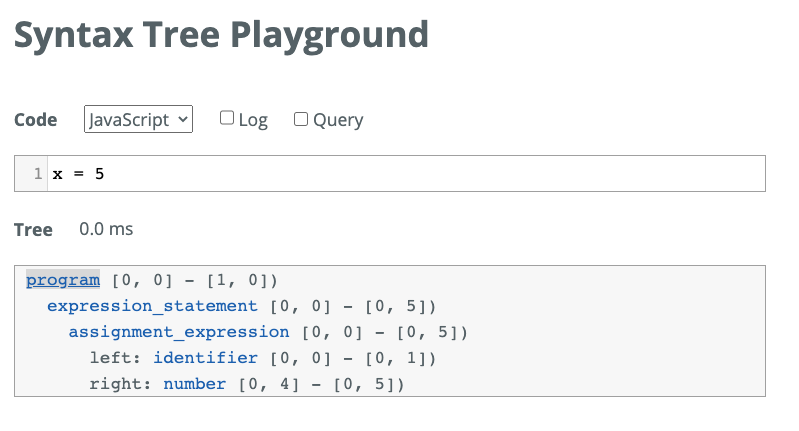
\includegraphics[width=0.8\linewidth]{images/playground.png}
    \caption{TreeSitter Playground}%
    \label{fig:playground}
\end{figure}

\subsection{Queries}%
\label{sub:queries}
TreeSitter provides an API for extracting pieces of a program that matches the patterns within a given query.
This makes it very simple to use TreeSitter to find and analyze parts of a program without having to manually
traverse the parse tree.
Query patterns are written as \textit{S-expressions} where the first element within the parentheses
is the type of node to match on, followed by zero or more patterns for the children of that node.
The following query consist of a single pattern that will match in a binary expression were both operands are number literals
such as \texttt{1 + 2}, but not \texttt{``hello '' + ``world''}:
\begin{verbatim}
(binary_expression (number) (number))
\end{verbatim}

Children of a particular node might have \textit{field names} assigned to them 
which can be used in the pattern.
For example, to match on binary expressions where the left-hand side is a number literal
one might write a query like:
\begin{verbatim}
(binary_expression left: (number))
\end{verbatim}

Captures can be introduced to store and organize the results of the query.
The following query would find all identifiers that occur on the left-hand side of an assignment,
and let you refer to them through the name \texttt{declared-variable}:
\begin{verbatim}
(assignment_expression left: (identifier) @declared-variable)
\end{verbatim}

Predicates allow query results to be filtered based on the value of the captured variables.
This makes TreeSitter queries a convenient way of searching for specific nodes in a program.
In addition to the \texttt{\#eq?} predicate for checking equality, there is the \texttt{\#match?} predicate
to match by regular expressions.
Listing~\ref{listing:queryX} shows a query that will find all occurrences of assigning a value to the variable named ``x'':
\begin{code}{text}{Query for Declarations of ``x''}{listing:queryX}
(
 (assignment_expression left: (identifier) @declared-variable)
 (#eq? @declared-variable "x")
)
\end{code}

\urldef\tsqueryurl\url{https://tree-sitter.github.io/tree-sitter/using-parsers\#pattern-matching-with-queries}
The query API is quite expressive and supports more featured than covered in this section\footnote{\tsqueryurl}.
% TODO: broken link




\section{Elm}\label{sec:elm}
In this thesis I will be using Elm as the subject of the analysis.
Elm is a feature rich, but relatively simple language.
The reason elm was chosen for this project is that it has a solid implementation of
the Language Server Protocol, a reliable TreeSitter parser, and its relative simplicity
makes it more realistic to achieve a high degree of completeness in the prototype.
Some knowledge of Elm is useful for the reader, but no experience is required.
This section will primarily cover the features of Elm that introduces new identifiers into the scope,
as these will be relevant when generating voice commands later.

\subsection{Introduction}
Elm is a statically typed, purely functional programming language for crating responsive web applications.
It is a member of the ML (\textit{Meta Language}) family of programming languages
and therefore resembles languages like Haskell and OCamel the most.


\subsection{Functions and Values}
The syntax for declaring top-level values and functions is very simple.
\Vref{ex:value_and_function} shows two declarations.
The first simply binds the value 5 to the identifier \texttt{five},
while the second defines a function that takes a number as an argument and increments it.
Both declarations are preceded by a type signature, both of which are completely optional
due to the fact that Elm has global type inference.
\begin{code}{elm}{Simple Value and Function Declaration}{ex:value_and_function}
five : Int
five = 5

increment : Int -> Int
increment number = number + 1
\end{code}
The syntax for functioning invocation is simply adjacency, so the expression
\textbf{increment five} would evaluate to \textbf{6}.

\textbf{Note:}
Since elm is a higher order language, functions are also normal values which is reflected
in how there is no separate syntax for declaring functions and values.
Also, since Elm does not support mutable variables there is no distinction
between terms like ``constant'', ``variable'' and ``value'' like there is in many languages.
% disambiguate this terminology. how will I use these words?
% This paper I will use the word ``'' to refer to non
% From a theoretical point of view, non-function values can be considered as
% functions of arity zero. For this reason, normal values 


\subsection{Types}
As in many ML languages, types are a central concept in Elm.
This section covers the central aspects of the Elm type system.
% \subsubsection{Built-in Types}
The language has a few basic types such as \texttt{Int}, \texttt{Float}, \texttt{Char} and \texttt{String}
which represents integers, floating-point numbers, characters and sequences of characters respectively.
Additionally there are a few special types.
\texttt{Never} is a type that has no values.
\texttt{()} is the unit type which has exactly one value.
Function types are denoted by an arrow (\texttt{->}).
If A and B are both types, a function that takes an A and returns a B would have the type (\texttt{A -> B})
which is commonly pronounced ``from A to B''.
The function arrow is right associative, meaning that \texttt{A -> B -> C} is the same as \texttt{A -> (B -> C)}.
There is also syntax for tuple types such as \texttt{(A, B)} or \texttt{(A, B, C)}
which represents pairs and triples.
% Unlike other ML languages like Haskell, Elm does not support tuples of lengths greater than three.

\subsubsection{Record Types}
Elm supports record types which are product types with named fields, similar to \textit{structs} in languages like \texttt{C}.
Records can have any number of fields, each of which can have any type.
A significant difference between Elm records and C structs is that Elm supports anonymous record types
meaning that they can be used without being given a name as seen in Listing~\ref{ex:anonymous}.
\begin{code}{elm}{Anonymous Records}{ex:anonymous}
john : { name : String, age : Int }
john = { name = "John", age = 25 }
\end{code}
Elm records are also extensible which means you can define a lower bound
for the fields a record needs to have.
The canonical example, seen in Listing~\ref{extensible}, is a type that describes records with at least a field \texttt{id} with the type \texttt{Int}.
\begin{code}{elm}{Extensible Records}{extensible}
type alias HasId r = { r | id : Int }
\end{code}




\subsubsection{User-defined Types}
There are two ways of declaring a new type:
\begin{enumerate}
    \item{``Normal'' Type Declarations} 
    \item{Type Alias Declarations} 
\end{enumerate}
Normal type declarations formally corresponds to \textit{Algebraic Data Types},
often simply referred to as ``union types'' or ``custom types''.
Type alias declarations corresponds to transparent type synonyms.
% Additionally, Elm has anonymous and extensible record types.

\paragraph{Type Aliases} are a way of introducing alternate names for existing types.
The use of type aliases does not affect how the program type checks, but can help improve readability.
Listing~\ref{position} shows how you can use a type alias to make what the function does more clear.
\begin{code}{elm}{Type Alias}{position}
type alias Position = (Int, Int) 

moveNorth : Position -> Position
moveNorth (x, y) = (x, y + 1)
\end{code}
Type aliases has a special property when interacting with records in Elm.
If a type alias is created for a record, a function with the same name as the type
is automatically created to act as a constructor for this record.
Given the declaration in Listing~\ref{record_alias}, a function \texttt{Person}
would be introduced with the type \texttt{String -> Int -> Person}.
This is often convenient when creating records with higher-order functions.
\begin{code}{elm}{Record Alias}{record_alias}
type alias Person =
    { name : String
    , age : Int
    }

john : Person
john = Person "John" 25
\end{code}

\paragraph{Union Types} are the main tool for data modeling in Elm.
\Vref{maybe} shows the definition of an important data type called \texttt{Maybe}
which is used to represent the possibility of absence of a value.
\texttt{Maybe} has two constructors, the first of which has one argument while the second has zero arguments.
The \texttt{a} in this example is a type variable which indicates that \texttt{Maybe} it is a polymorphic type.
When this type has been defined, \texttt{Nothing} is a constant value of type \texttt{Maybe}, and \texttt{Just}
is a function with the type \texttt{a -> Maybe a}, so \texttt{Maybe}-values can be created
with expressions such as \texttt{Nothing}, \texttt{Just 5} or \texttt{Just ``hello''} and so on.
\begin{code}{elm}{The \texttt{Maybe} Union Type}{maybe}
type Maybe a
    = Just a
    | Nothing
\end{code}

\textbf{Note:}
The word ``constructors'' has special meaning in some languages, but in Elm they
are normal functions and have no special properties in the language
except that their names start with an uppercase letter which makes them syntactically distinct
from other functions.

\subsubsection{Polymorphism}
Elm supports regular \textit{parametric polymorphism} (also known as \textit{generics} in object-oriented programming)
as seen in \Vref{maybe} which defined a polymorphic container, and \Vref{ex:polymorphic_function}
which defines a polymorphic function.
The language does not support higher ranked types.
Additionally Elm supports a limited form of ad hoc polymorphism.
In order to overload operators such as \texttt{(+)}, \texttt{(<)} and \texttt{(++)}
there are special type variables called \textit{Constrained Type Variables}.
\Vref{ctv} shows the name of these special variables along with the
concrete types they are compatible with.

\begin{table}[htpb]
    \centering
    \begin{tabular}{c|c}
        % \toprule
        % \hline
        Name & Permits \\
        \hline
        number & Int, Float \\
        appendable & String, List \texttt{a} \\
        comparable & number, Char, String, (List|Tuple) \texttt{comparable} \\
        compappend & String, List \texttt{comparable} \\
        % \hline
        % \bottomrule
    \end{tabular}
    \caption{Constrained Type Variables}
    \label{ctv}
\end{table}
\begin{code}{elm}{Polymorphic Function}{ex:polymorphic_function}
{-| Swaps the elements of a tuple -}
swap : (a, b) -> (b, a)
swap (a, b) = (b, a)
\end{code}

\subsection{Modules and Imports}
Elm code is organized into modules which are used to organize projects
and separate code into different name spaces.
Each file starts with a module declaration which contains the name of the module (which must start with an uppercase letter)
and the list of members to be exposed.
Elm does not use visibility modifiers such as \texttt{public/private}, as they do in languages
like Java, but elements of the exposing list are available to other modules through imports.
An example of a module declaration and import statements can be seen in the first few lines of \Vref{listing:elm_simple}.
When importing a module you can optionally provide an alias with the \texttt{as}-keyword
and/or an exposing list.
After a module has been imported, exposed members of that module can be accessed
through its name and a dot (\texttt{.}) as in \texttt{Browser.sandbox}.
Import aliases provides an alternate name for referring to the module within the current one
which is convenient for modules with long names.
Members included in the exposing list of an important statement can be used directly
without prefixing it with the module name.

\subsubsection{The Exposing List}
There are four types of items that can occur in the exposing list.
Lowercase identifiers always refers to variables in the module.
Uppercase identifiers always refers to a type.
The double dot token (\texttt{..}) means to include everything in the module.
An uppercase identifier followed by a double dot refers to a type as well as all the constructors on that type.

\subsection{Namespaces}
Most programming languages store identifiers in different name spaces, which allows a single name
to refer to multiple constructs in the language.
Elm has separate name spaces for modules, functions, and types.
As a consequence, the identifier ``String'' may refer to the \texttt{String} module in \texttt{elm/core}, or the \texttt{String} type.

    
\begin{code}{elm}{Simple Elm Program}{listing:elm_simple}
module Main exposing (Model, Msg(..), init, main, update, view)

import Browser
import Html exposing (Html, button, div, text)
import Html.Events as Events exposing (onClick)

-- MAIN

main =
    Browser.sandbox { init = init, update = update, view = view }

-- MODEL

type alias Model = Int

init : Model
init = 0

-- UPDATE

type Msg
    = Increment
    | Decrement

update : Msg -> Model -> Model
update msg model =
    case msg of
        Increment ->
            model + 1

        Decrement ->
            model - 1

-- VIEW

view : Model -> Html Msg
view model =
    div []
        [ button [ onClick Decrement ] [ text "-" ]
        , div [] [ text (String.fromInt model) ]
        , button [ onClick Increment ] [ text "+" ]
        ]
\end{code}

